\documentclass[10pt, a4paper, oneside]{article}
\usepackage[hidelinks]{hyperref}
\usepackage{jucs2e}
\usepackage{graphicx}
\usepackage{url}
\usepackage[normalem]{ulem}
\usepackage{mathtools}
\usepackage{amssymb}
\usepackage{scalerel}
\usepackage{setspace}
\usepackage[strict]{changepage}
\usepackage{caption}
\usepackage[letterspace=-50]{microtype}
\usepackage{fontspec}
\usepackage{afterpage}
\usepackage{ragged2e}
\usepackage{booktabs}

\setmainfont{Times New Roman}

\usepackage{titlesec}

\titleformat*{\section}{\Large\bfseries}
\titleformat*{\subsection}{\normalsize\bfseries}

\renewcommand{\baselinestretch}{0.9}

\graphicspath{{./figures/}}

\usepackage[textwidth=8cm, margin=0cm, left=4.6cm, right=4.2cm, top=3.9cm, bottom=6.8cm, a4paper, headheight=0.5cm, headsep=0.5cm]{geometry}
\usepackage{fancyhdr}
\usepackage[format=plain, labelfont=it, textfont=it, justification=centering]{caption}
% Pies de figura y tabla: 10 pt cursiva con 11 pt de interlineado y 12 pt antes y despues, como indica la plantilla
\DeclareCaptionFont{jucscap}{\fontsize{10pt}{11pt}\selectfont}
\captionsetup{font=jucscap, skip=12pt, belowskip=0pt}
% jucs2e.sty fija \belowcaptionskip en -10pt, lo que monta el pie de una figura sobre el de la tabla siguiente
\setlength{\belowcaptionskip}{0pt}
\setlength{\floatsep}{16pt plus 2pt minus 2pt}
\setlength{\textfloatsep}{16pt plus 2pt minus 2pt}
\setlength{\intextsep}{16pt plus 2pt minus 2pt}
\usepackage{breakcites}
\usepackage{microtype}

\apptocmd{\frame}{}{\justifying}{}

\urlstyle{same}
\pagestyle{fancy}

\newcommand\jucs{{Journal of Universal Computer Science}}
\newcommand\jucsvol{vol. --, no. -- (----)}
\newcommand\jucspages{--}
\newcommand\jucssubmitted{--}
\newcommand\jucsaccepted{--}
\newcommand\jucsappeared{--}
\newcommand\jucslicence{ CC BY 4.0}
\newcommand\startingPage{1}
\setcounter{page}{\startingPage}

%Author
\newcommand\paperauthor{{Aviles-Esparza J. P. et al.: }}

% Title
\newcommand\papertitle{Concept Drift in URL-Based Phishing Detection: A Temporal Evaluation}

% Main header content
\header{\paperauthor \papertitle}
% La cabecera de paginas pares de jucs2e.sty trae fijo el texto de ejemplo de la plantilla;
% se redefine aqui con los autores y el titulo de este articulo.
\fancyhead[OC]{%
  {\ifnum\thepage=\startingPage
  \begin{singlespace}
      \fontsize{8pt}{5pt}\selectfont{\itshape{\jucs, \jucsvol, \jucspages \\ submitted: \jucssubmitted, accepted: \jucsaccepted, appeared: \jucsappeared \jucslicence}}
      \vspace{-5mm}
  \end{singlespace}
  \else
      \lsstyle
      {\fontsize{8pt}{5pt}\selectfont{\itshape{Aviles-Esparza J. P. et al.: Concept Drift in URL-Based Phishing Detection}}}
      \vspace{-0.5mm}
  \fi}}

\begin{document}

\title{{\fontsize{14pt}{14pt}\selectfont{\vspace*{-3mm}\papertitle\vspace*{-1mm}}}}

\author{{\bfseries\fontsize{10pt}{10pt}\selectfont{Juan Pablo Aviles-Esparza*}} \\
   {\fontsize{9pt}{12pt}\selectfont{(Escuela Superior Polit\'ecnica de Chimborazo, Riobamba, Ecuador\\
   \orcid{0009-0007-0058-8069}, 
   juan.aviles@espoch.edu.ec)}}
   \and
   {\bfseries\fontsize{10pt}{10pt}\selectfont{Italo Javier Tenempaguay-Granizo}} \\
   {\fontsize{9pt}{12pt}\selectfont{(Escuela Superior Polit\'ecnica de Chimborazo, Riobamba, Ecuador\\
   \orcid{0009-0001-5753-4279}, 
   italo.tenempaguay@espoch.edu.ec)}}
   \and
   {\bfseries\fontsize{10pt}{10pt}\selectfont{Isaac David Torres-Paredes}} \\
   {\fontsize{9pt}{12pt}\selectfont{(Escuela Superior Polit\'ecnica de Chimborazo, Riobamba, Ecuador\\
   \orcid{0009-0001-7057-9316}, 
   isaac.torres@espoch.edu.ec)}}
}

\label{first}
\maketitle

{\fontfamily{ptm}\selectfont
\begin{abstract}
{\fontsize{9pt}{9pt}\selectfont{\vspace*{-2mm}
Phishing detectors are almost universally evaluated with random train/test splits, which implicitly assume that a URL's characteristics are exchangeable across time. We test that assumption by training three lexical-feature classifiers (random forest, XGBoost, logistic regression) on 180 days of PhishTank-reported phishing URLs plus an equal number of legitimate domains from the Tranco ranking, and evaluating them under four designs: a random split, training on the earliest block and testing on each later block, a sliding retraining window, and cumulative retraining. All three models achieve F1 above 0.98 in every configuration, and the gap between the random-split baseline and the worst temporally displaced block is small (0.36 to 0.92 percentage points of F1). All three models decline with temporal distance, but with the evaluation block as the independent unit the trend is not significant (Spearman $\rho=-0.70$, $p=0.19$, five blocks; $\rho=-0.44$, $p=0.18$, eleven blocks), so we report it as consistent in direction but weakly supported. The near-ceiling performance reflects how the data were built: legitimate URLs are bare domains, and removing the four features tied to URL shape (\texttt{is\_https}, \texttt{path\_length}, \texttt{num\_slashes}, \texttt{url\_length}) lowers F1 by 3.3 to 4.2 points, whereas removing four other important features lowers it by at most 0.4. Because PhishTank's feed lists only phishing that is still online, older phishing is under-represented and the phishing share per block rises from 25\% to 62\%; prevalence-independent metrics show the same pattern. Temporal evaluations of phishing detection need a negative class of full legitimate URLs with real timestamps.}}
\end{abstract}}

{\fontfamily{ptm}\selectfont
\begin{keywords}
{\fontsize{9pt}{9pt}\selectfont{
Phishing detection, Concept drift, Temporal evaluation, Lexical features, Machine learning, Cybersecurity}}
\end{keywords}}

{\fontfamily{ptm}\selectfont
\begin{category}
{\fontsize{9pt}{9pt}\selectfont{
C.2.0, I.2.6, I.5.2, K.6.5}}
\end{category}}

{\fontfamily{ptm}\selectfont
\begin{doi}
{\fontsize{9pt}{9pt}\selectfont{
10.3897/jucs.\textless SubmissionNumber\textgreater}}
\end{doi}}

{\fontsize{9pt}{11pt}\selectfont *Corresponding author.}

\section{Introduction}

Phishing is an adversarial instance of the broader concept-drift problem in machine learning \cite{gama2014survey}: attackers change URL patterns, hosting infrastructure, and lexical tricks specifically to evade whatever a detector has already learned to flag. A classifier trained and evaluated with a single random train/test split treats every URL in the dataset as drawn from one stationary distribution, which is precisely the assumption an adversarial, evolving threat violates. If that assumption is wrong, published accuracy figures based on random splits systematically overstate what a detector will achieve once deployed against future, unseen phishing campaigns.

This paper asks how large that gap is, using a temporal evaluation design instead of a random one, and compares two common mitigation strategies, periodic retraining with a sliding window versus cumulative retraining that keeps all historical examples, to see whether either meaningfully closes it. We evaluate on 180 days of continuously reported phishing URLs, which lets us construct time-ordered evaluation blocks instead of simulating drift artificially.

The contributions of this work are: (1) a temporal, block-based evaluation of lexical phishing classifiers on real, timestamped data, contrasted directly against the random-split baseline the field defaults to; (2) a statistical treatment of the degradation trend that contrasts model-level tests (ANCOVA, Page test) with inference that treats the evaluation block as the independent unit, showing that the trend is consistent in direction but weakly supported; (3) an account, based on feature distributions, feature importance, and an ablation with a control feature set, of why the measured degradation is small: an easy negative class, built from bare domains, not a solved drift problem.

\section{Related Work}

Odeh et al. \cite{odeh2021phiboost} propose PhiBoost, an adaptive-boosting phishing detector that selects the features most correlated with the class label, and report accuracy of approximately 99\% on a static dataset; a time-agnostic evaluation of this kind is the protocol this paper argues is insufficient on its own, since it cannot distinguish a detector that has learned durable phishing indicators from one that has overfit to the particular campaigns present in the training window. Sahingoz et al. \cite{sahingoz2019phishing} benchmark seven classifiers on natural-language-processing features extracted from URLs, with Random Forest (also the strongest model in our study) performing best at close to 98\% accuracy; because their features are also URL-based, the temporal gap we measure bears directly on how such baselines should be read, rather than on the choice of classifier. Concept drift in adversarial text classification has also been studied for spam: Henke et al. \cite{henke2021spam} detect drift by comparing the feature vectors extracted from training and test data, and transfer knowledge between models when the features evolve, which is the kind of feature-level shift we examine for phishing URLs (Discussion). Our temporal blocks follow the block-based evaluation used in data-stream classification; Kozal et al. \cite{kozal2022chunk} show that the size of those blocks affects how quickly a classifier recovers after a drift, which is one reason we repeat the block-level analysis with twelve blocks as well as six. Duraz et al. \cite{duraz2024cvss} argue that intrusion detection systems should be evaluated with metrics that reflect the severity of the attacks, not with accuracy alone; our use of prevalence-independent metrics responds to a related concern about how evaluation choices shape the performance a detector appears to have. On the human side, Crgol and Vrhovec \cite{crgol2024phishing} find that recognising phishing emails in a survey is not associated with how people respond to a real phishing campaign, which motivates automated detection that does not depend on user judgement.

This concern is not new to security classification in general: Pendlebury et al. \cite{pendlebury2019tesseract} name and formalize the same failure mode for malware classifiers under the label \emph{temporal bias}, showing that a naive random train/test split can silently mix future and past samples and thereby overstate real-world performance, and propose constraints for avoiding it: training strictly on data older than the test data, testing with a realistic ratio between the classes, and drawing both classes from the same time windows. Our fixed, sliding-window, and cumulative designs satisfy the first constraint by construction but not the other two, because the dataset is balanced overall and the legitimate class carries synthetic timestamps (Limitations). The phishing URL studies reviewed below evaluate on static or randomly split data, so the temporal question is the gap this paper addresses. Jemili et al. \cite{jemili2024ids} address concept drift in network intrusion detection by combining a drift-detection method with an online random forest that is updated incrementally, evaluated on the MAWILab traffic data; their work treats drift as a practical concern in security classification streams, but they do not study lexical URL features or control for the contribution of class-boundary difficulty to the observed gap, which is the mechanistic question we pursue here. Apruzzese et al. \cite{apruzzese2023real} examine the gap between adversarial machine-learning research and operational practice and argue, from real-world case studies, that actual attackers mostly use simple tactics rather than the algorithmic attacks studied in the literature. If so, random-split evaluations are unrealistic in two ways: in their time ordering and in the adversarial capability they assume. We take that as additional motivation for a design that at least corrects the temporal dimension, even if it does not resolve the adversarial-realism dimension.

At the survey level, Buczak and Guven \cite{buczak2016survey} review machine-learning and data-mining methods for intrusion detection, describe the data sets commonly used to evaluate them, and discuss the challenges of applying these methods in cyber security; they do not compare retraining strategies under temporal separation, which is the comparison our study provides for phishing URLs (fixed, sliding-window, and cumulative retraining). Varshney, Misra and Atrey \cite{varshney2016phishing} provide a complementary survey and classification of web phishing detection schemes; our study concerns URL-based (lexical) detection only and asks an empirical question such surveys do not settle: whether lexical-only detectors maintain their reported accuracy as the phishing population changes over time.

The feature-engineering and modelling approaches evaluated in this paper have direct precedents in the phishing-detection literature. Mohammad, Thabtah and McCluskey \cite{mohammad2014phishing} introduce an intelligent rule-based classifier for phishing websites using URL and page-level features, and in a companion study \cite{mohammad2013neural} apply self-structuring neural networks to the same feature family; both are evaluated on static datasets, which places their results closest to the random-split condition in our design and makes them subject to the same temporal-bias concern that Pendlebury et al. \cite{pendlebury2019tesseract} formalize for malware and that we quantify here for phishing. Singh and Meenu \cite{singh2020phishing} survey machine-learning approaches to phishing website detection from URLs; whether the performance such detectors report holds as phishing changes over time is the gap this paper addresses. Somesha et al. \cite{somesha2020phishing} apply deep-learning architectures to phishing website detection and report very high accuracy; in our lexical-feature setting, comparatively simple tree ensembles already reach F1 above 0.99, with Random Forest the strongest model in all four temporal designs. Hannousse and Yahiouche \cite{hannousse2021benchmark} construct benchmark datasets for machine-learning-based website phishing detection and argue that results depend on how such datasets are built; our ablation gives one concrete instance of that dependence, with the features most tied to how the Tranco-derived legitimate class was constructed accounting for 3.3 to 4.1 F1 points (Results, Table~\ref{tab:ablation}).


\section{Methodology}

\subsection{Data}
Phishing URLs were drawn from PhishTank's public feed, which is the only phishing source we found that ships a reliable, unauthenticated \texttt{submission\_time} timestamp per URL (OpenPhish's community feed and the static UCI Phishing Websites / PhiUSIIL datasets do not carry a comparable per-record date and were excluded from this design for that reason). We retained the submissions of the most recent 180 days, from 20 February to 19 August 2026 (29{,}299 URLs). PhishTank's downloadable feed lists only verified phishing that is still online (every record in our download has \texttt{online} = yes), so phishing reported earlier and already taken down is missing: older weeks contain fewer surviving URLs, and those that survive are likely to be longer-lived than average. Legitimate URLs were sampled from the Tranco top-1M list \cite{lepochat2019tranco} , chosen over alternatives such as the (now-discontinued) Alexa ranking because Tranco is designed to resist the list-manipulation attacks that make raw popularity rankings an unreliable ground truth for security research. Tranco lists domains, not URLs; each sampled domain was turned into a URL by prefixing \texttt{http://} with no path, so every legitimate URL has \texttt{is\_https} $=0$ and \texttt{path\_length} $=0$, whereas 83.4\% of the phishing URLs use \texttt{https}. This asymmetry is examined in the ablation (Discussion). Because Tranco is a single ranked snapshot rather than a dated feed, each sampled legitimate URL was assigned a synthetic timestamp drawn uniformly over the same 180-day window as the phishing data, a deliberate simplification justified because domain reputation for an established, highly ranked site does not meaningfully change on a 180-day horizon, in contrast to phishing infrastructure, which is exactly what this study measures as changing. The final dataset is balanced overall (29{,}299 phishing, 29{,}299 legitimate) but not within temporal blocks: because surviving phishing becomes more frequent towards the end of the window while legitimate timestamps are uniform, the phishing share of the six blocks is 24.8, 45.2, 52.4, 58.3, 57.0, and 62.4\%. Duplicate URLs were not present, but 17{,}637 rows (30.1\%) repeat another row's feature vector, mostly in the legitimate class; they were kept in the main analysis, and repeating the random split without them changes F1 by at most 0.0010.

\subsection{Features}
We extract 32 lexical features per URL requiring no live network access (URL/hostname/path length, counts of dots/hyphens/digits/special characters, subdomain count, IP-literal hostname flag, presence of a known URL shortener, Shannon entropy of the URL and hostname strings, a count of phishing-associated keywords, and related structural features). Table~\ref{tab:features} lists all 32 with their definitions. Features were standardised with a scaler fitted on the full dataset; refitting it on each training set alone changes logistic regression's mean fixed-design F1 from 0.9899 to 0.9911 and leaves the two tree ensembles unchanged to the third decimal.

\begin{table}[htbp]
\centering
\footnotesize
\caption{Lexical features extracted per URL.}
\label{tab:features}
\begin{tabular}{ll}
\toprule
Feature & Definition \\
\midrule
\texttt{url\_length} & Character length of the full URL \\
\texttt{hostname\_length} & Character length of the hostname \\
\texttt{path\_length} & Character length of the URL path \\
\texttt{num\_dots} & Count of \texttt{.} characters in the URL \\
\texttt{num\_hyphens} & Count of \texttt{-} characters in the URL \\
\texttt{num\_underscores} & Count of \texttt{\_} characters in the URL \\
\texttt{num\_slashes} & Count of \texttt{/} characters in the URL \\
\texttt{num\_question\_marks} & Count of \texttt{?} characters in the URL \\
\texttt{num\_equals} & Count of \texttt{=} characters in the URL \\
\texttt{num\_at} & Count of \texttt{@} characters in the URL \\
\texttt{num\_ampersands} & Count of \texttt{\&} characters in the URL \\
\texttt{num\_percent} & Count of \texttt{\%} characters in the URL \\
\texttt{num\_digits} & Count of digit characters in the URL \\
\texttt{digit\_ratio} & Digit characters as a fraction of URL length \\
\texttt{num\_subdomains} & Number of hostname labels beyond domain and TLD \\
\texttt{has\_ip\_address} & 1 if the hostname is a literal IPv4 address \\
\texttt{has\_port} & 1 if a port number is present \\
\texttt{is\_https} & 1 if the scheme is \texttt{https} \\
\texttt{url\_entropy} & Shannon entropy of the full URL string \\
\texttt{hostname\_entropy} & Shannon entropy of the hostname string \\
\texttt{is\_shortened} & 1 if hostname matches a known URL-shortener domain \\
\texttt{num\_suspicious\_keywords} & Count of phishing-associated keywords (e.g., ``login'', ``verify'') \\
\texttt{has\_suspicious\_keyword} & 1 if any suspicious keyword is present \\
\texttt{domain\_length} & Character length of the second-level domain label \\
\texttt{path\_num\_segments} & Number of non-empty path segments \\
\texttt{has\_double\_slash\_in\_path} & 1 if \texttt{//} appears inside the path \\
\texttt{num\_www} & 1 if the hostname starts with \texttt{www.} \\
\texttt{longest\_label\_length} & Length of the longest hostname label \\
\texttt{tld\_length} & Character length of the top-level domain \\
\texttt{has\_at\_symbol} & 1 if \texttt{@} appears anywhere in the URL \\
\texttt{num\_dashes\_in\_hostname} & Count of \texttt{-} characters within the hostname only \\
\texttt{vowel\_ratio\_hostname} & Vowel characters as a fraction of hostname length \\
\bottomrule
\end{tabular}
\end{table}

\subsection{Temporal evaluation designs}
Data were sorted by timestamp and divided into six blocks of equal sample count (not of equal class composition; see Data). We evaluate four designs: (i) \emph{random}, an 80/20 random split ignoring time, as a baseline; (ii) \emph{fixed}, training once on block 1 and evaluating separately on blocks 2 through 6, to isolate pure degradation with distance; (iii) \emph{sliding window}, training on block $k$ and evaluating on block $k+1$ for each consecutive pair, simulating periodic retraining on only the most recent data; (iv) \emph{cumulative}, training on blocks $1$ through $k$ and evaluating on block $k+1$, simulating retraining that keeps the full history. All models (random forest \cite{breiman2001random}, XGBoost \cite{chen2016xgboost}, logistic regression) share identical standardized features across designs.

\subsection{Statistical analysis}
We regress F1 on temporal distance for the fixed design, per model, pooled naively across models, and pooled with a model fixed effect (ANCOVA: \texttt{f1 \textasciitilde{} distance + model}) to separate the within-model trend with distance from the large between-model differences in baseline F1, which a naive pooled regression otherwise folds into its residual variance and thereby understates the trend's significance. Because a linear regression with only three models provides limited power to detect a common monotonic trend regardless of specification, we additionally run a Page test for a monotonic decreasing trend, treating the three models as judges ranking the five temporal-distance conditions, and cross-check its normal-approximation $p$-value with a Monte Carlo permutation null (100,000 iterations). Both tests treat the three models as independent replicates, but the models are evaluated on the same blocks and share each block's difficulty, so the block is the independent unit. We therefore also test the trend with Spearman's correlation between temporal distance and the mean F1 of the three models per block, with six blocks and, as a sensitivity check, with twelve; and we repeat it with metrics that do not depend on class prevalence (true-positive rate, false-positive rate, balanced accuracy, and F1 on evaluation blocks rebalanced to 50/50 by subsampling the majority class, 20 repetitions). We compare the sliding-window and cumulative strategies with a paired bootstrap over the predictions of each evaluation block (2{,}000 resamples per block, pooled across the five blocks) as the main test, and report the paired Wilcoxon signed-rank test per model for completeness.

\subsection{Use of generative AI tools}
The authors used Claude (Anthropic; models Claude Sonnet~5 and Claude Opus~5.5) as an assistant for language editing, for support in writing and debugging the analysis code, and for LaTeX formatting. The research questions, study design, data collection, execution of the analyses, results, and their interpretation are the authors' own work; all AI-assisted output was reviewed and verified by the authors, who take full responsibility for the content of this article. No figure was produced with image-generation tools.

\section{Results}

All three models achieve F1 $>0.98$ in every one of the four designs: there is no configuration in which any model performs poorly in absolute terms (Figure~\ref{fig:degradacion}). In relative terms, Table~\ref{tab:degradation} shows the gap between the random-split baseline and the temporally displaced (fixed-design) evaluations is small (0.09 to 0.35 percentage points of F1 on average across displaced blocks, model-dependent) but non-zero, and grows toward the worst-case block (up to 0.92 points for logistic regression); Table~\ref{tab:f1-by-block} gives the full breakdown by block and model.

\begin{table}[h]
\centering
\caption{F1 under random vs.\ temporal (fixed-training) evaluation.}
\label{tab:degradation}
\begin{tabular}{lccc}
\toprule
Model & F1 (random split) & F1 (temporal, avg.) & F1 (temporal, worst block) \\
\midrule
Random Forest        & 0.9952 & 0.9943 & 0.9916 \\
XGBoost               & 0.9951 & 0.9935 & 0.9902 \\
Logistic Regression   & 0.9934 & 0.9899 & 0.9842 \\
\bottomrule
\end{tabular}
\vspace{4pt}
\caption*{\small \textit{Note: The random split trains on 80\% of the full dataset, whereas the fixed-training temporal design trains on roughly one-sixth (block 1 alone). Averages are computed from unrounded values, so they can differ in the last digit from the mean of the rounded entries in Table~\ref{tab:f1-by-block}.}}
\end{table}

\begin{figure}[h]
\centering
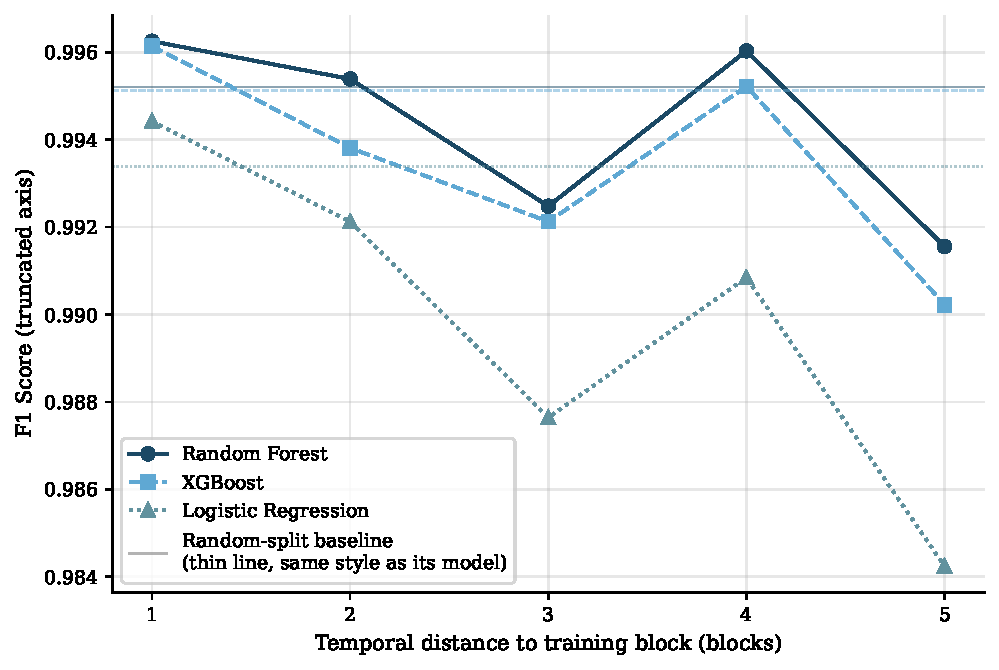
\includegraphics[width=0.75\textwidth]{figures/fig1_curva_degradacion.pdf}
\caption{F1 as a function of temporal distance (fixed-training design); thin horizontal lines mark each model's random-split baseline. The vertical axis is truncated to the range of the data.}
\label{fig:degradacion}
\end{figure}

\begin{table}[h]
\centering
\caption{F1 by evaluation block and model (fixed-training design: trained on block 1, evaluated on blocks 2 through 6, at increasing temporal distance).}
\label{tab:f1-by-block}
\setlength{\tabcolsep}{9pt}\begin{tabular}{lccc}
\toprule
Distance & Random Forest & XGBoost & Logistic Regression \\
\midrule
1 (block 2) & \textbf{0.9963} & 0.9961 & 0.9944 \\
2 (block 3) & \textbf{0.9954} & 0.9938 & 0.9921 \\
3 (block 4) & \textbf{0.9925} & 0.9921 & 0.9876 \\
4 (block 5) & \textbf{0.9960} & 0.9952 & 0.9908 \\
5 (block 6, worst) & \textbf{0.9916} & 0.9902 & 0.9842 \\
\bottomrule
\end{tabular}
\end{table}

A per-model OLS regression of F1 on temporal distance is directionally negative for all three models but reaches significance only for the pooled fit ($\beta = -0.00136$, $p = 0.022$, $R^2=0.34$); individually, logistic regression is marginal ($p=0.062$) and the two tree ensembles are not significant on their own ($p=0.25$ and $p=0.19$). This naive pooled fit, however, conflates two different sources of variance: the large, fixed differences in baseline F1 between models (logistic regression trails the two tree ensembles by roughly a full percentage point throughout) and the within-model trend with distance that is the actual quantity of interest. Controlling for model as a fixed effect (ANCOVA) removes the former from the residual: the slope estimate is unchanged ($\beta=-0.00136$, since the design is balanced across models) but its precision improves substantially ($p=0.0048$, $R^2=0.69$), because the between-model noise that was inflating the naive test's residual variance is no longer attributed to the distance trend. We treat the Page test as a further, specification-free check of the same conclusion: treating the three models as judges ranking F1 across the five temporal-distance conditions, the test rejects the null of no consistent ordering ($L=112$, $Z=-2.66$, $p=0.004$, one-sided). While there is a visible non-monotonic spike at distance 4 (block 5) for all three models (Figure~\ref{fig:degradacion}), the Page test is sensitive to overall ordinal trend rather than requiring strict monotonicity at every step, making it an appropriate contrast here. With only three judges, the test's normal approximation is known to have limited power and reliability, so we additionally computed an exact Monte Carlo permutation null (100,000 iterations, independently permuting each model's ranking across the five conditions under the null of no association between rank and temporal distance): the permutation-based $p$-value ($p=0.0026$, one-sided) agrees closely with, and is if anything slightly more extreme than, the asymptotic estimate, so the small-sample caveat does not change the conclusion. These three tests, however, treat the three models as independent replicates, and they are not: the models are evaluated on the same blocks, and the dip at block 4 and the spike at block 5 appear in all three, which indicates that block difficulty is shared. With the block as the unit, the mean F1 of the three models falls from 0.9958 at distance 1 to 0.9893 at distance 5, but the Spearman correlation is not significant ($\rho=-0.70$, $p=0.19$, two-sided, $n=5$); splitting the data into twelve blocks gives the same picture ($\rho=-0.44$, $p=0.18$, $n=11$). The prevalence-independent metrics give identical block-level correlations ($\rho=-0.70$ for balanced accuracy, rebalanced F1, and true-positive rate), so the rising phishing share across blocks does not drive the pattern; the decline comes from the true-positive rate (0.992 to 0.979), while the false-positive rate stays below 0.001. We therefore read the trend as consistent in direction across models and metrics but weakly supported: the model-level tests overstate the evidence, and five or eleven blocks are too few to establish it.

Comparing mitigation strategies, cumulative retraining outperforms sliding-window retraining for every model (Random Forest: 0.9952 vs.\ 0.9950; XGBoost: 0.9945 vs.\ 0.9939; Logistic Regression: 0.9931 vs.\ 0.9923) (Figure~\ref{fig:estrategias}); a size-matched control (Limitations) shows this advantage is mostly, and for logistic regression entirely, a consequence of cumulative retraining's larger training-set size, so we do not read this comparison as evidence that history itself is broadly beneficial. The paired bootstrap over the underlying predictions (Methods) finds the cumulative advantage for all three models, with 95\% confidence intervals excluding zero (Random Forest: $+0.00024$, 95\% CI $[0.00011, 0.00040]$; XGBoost: $+0.00067$, 95\% CI $[0.00035, 0.00099]$; Logistic Regression: $+0.00080$, 95\% CI $[0.00051, 0.00109]$; all $p<0.001$); the Wilcoxon test on five pairs per model cannot reach significance ($p=0.125$--$0.25$). The bootstrap resamples predictions of a single trained model per block, so its intervals do not include variability from training (for example, the random seed). The effect is small in absolute F1 terms, consistent with the modest overall degradation reported above.

\begin{figure}[h]
\centering
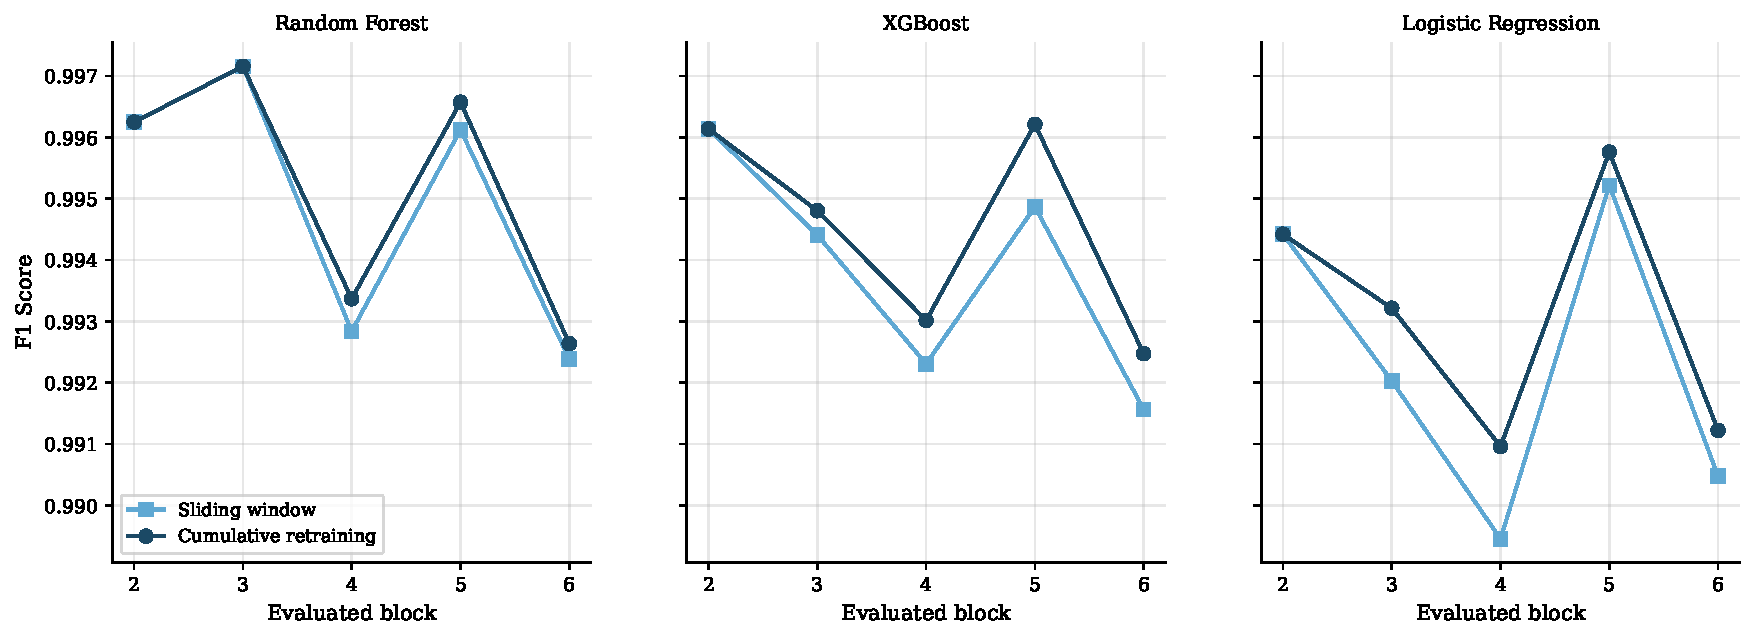
\includegraphics[width=0.85\textwidth]{figures/fig2_comparacion_estrategias.pdf}
\caption{F1 under sliding-window vs.\ cumulative retraining, by model and evaluated block (blocks 2--6).}
\label{fig:estrategias}
\end{figure}

\section{Discussion}

Degradation with temporal displacement is consistent in direction but small and weakly supported, far smaller than the field's framing of concept drift as a first-order threat would suggest. We think this is largely explained by the design of the negative class, not by the phishing detection task being inherently easy: our legitimate URLs come from Tranco's top-ranked, long-established domains, whose lexical signature (short, clean hostnames, no IP literals, low entropy, absence of phishing-associated keywords) is so different from phishing URLs that almost any reasonable classifier separates the two classes with ease, and that separation does not depend much on which specific phishing campaigns happen to be in the training set. A harder, more realistic negative class, such as legitimate URLs on recently registered or low-ranked domains, the same kind of short-lived infrastructure phishers register for their sites \cite{agarwal2026phishing}, or domains with URL structures that superficially resemble phishing (long paths, subdomains, marketing redirect chains), would very plausibly show a larger temporal gap, because the decision boundary would then depend more on the specific lexical tricks currently in fashion among phishers than on the broad, temporally stable distinction between an established domain and an ad hoc one. Recent large-scale evidence is consistent with this: Agarwal and Vasek \cite{agarwal2026phishing} analyse 15{,}126 domains registered solely to host phishing, with an average lifetime of 8.6 days, alongside compromised legitimate sites as the other main route; such short-lived domains are by construction absent from top-site rankings like Tranco, so an evaluation whose negatives are all top-ranked domains is likely to understate how hard the task is in operation.

\begin{figure}[h]
\centering
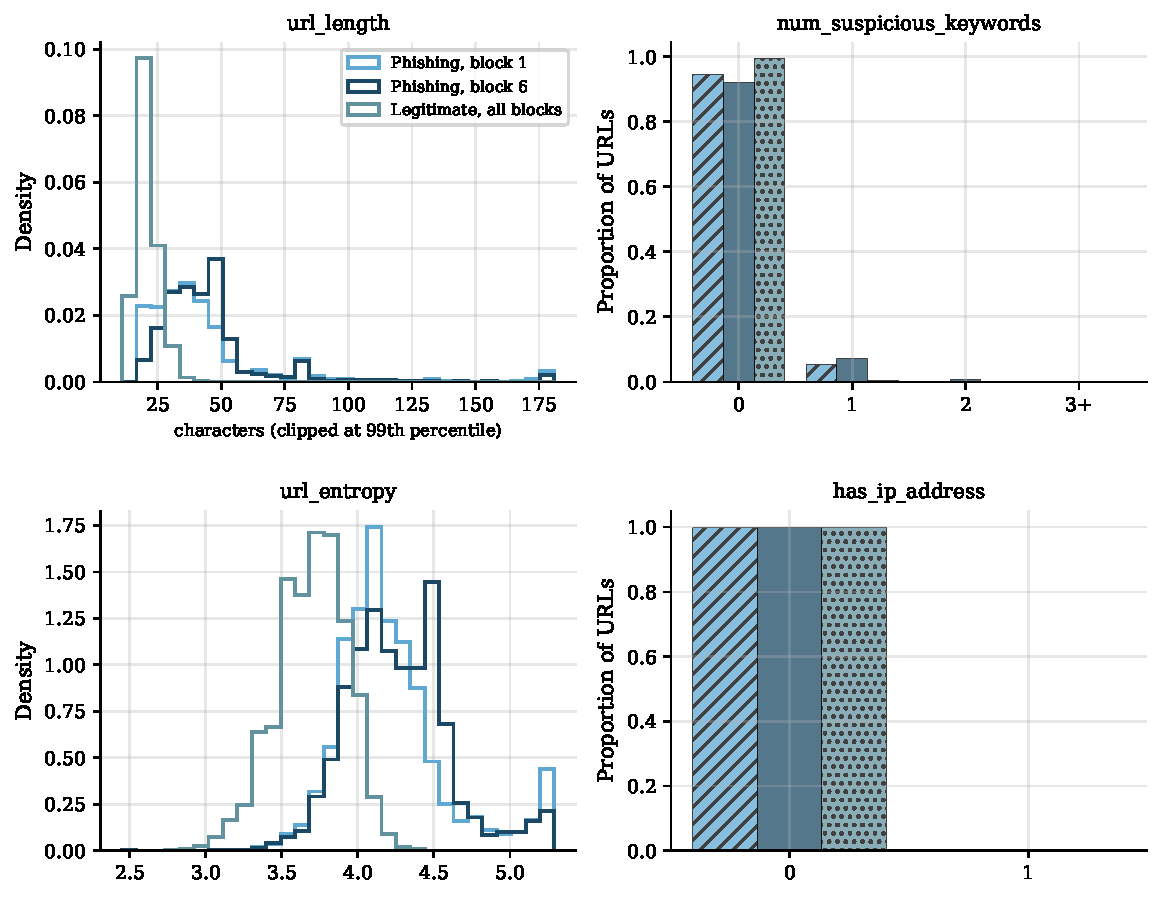
\includegraphics[width=0.8\textwidth]{figures/fig3_desplazamiento_features.pdf}
\caption{Distribution of four key lexical features among phishing URLs in the earliest and latest temporal blocks, with the legitimate class as reference. Continuous features are shown as densities (\texttt{url\_length} clipped at its 99th percentile); count and binary features as proportions.}
\label{fig:desplazamiento}
\end{figure}

\begin{figure}[h]
\centering
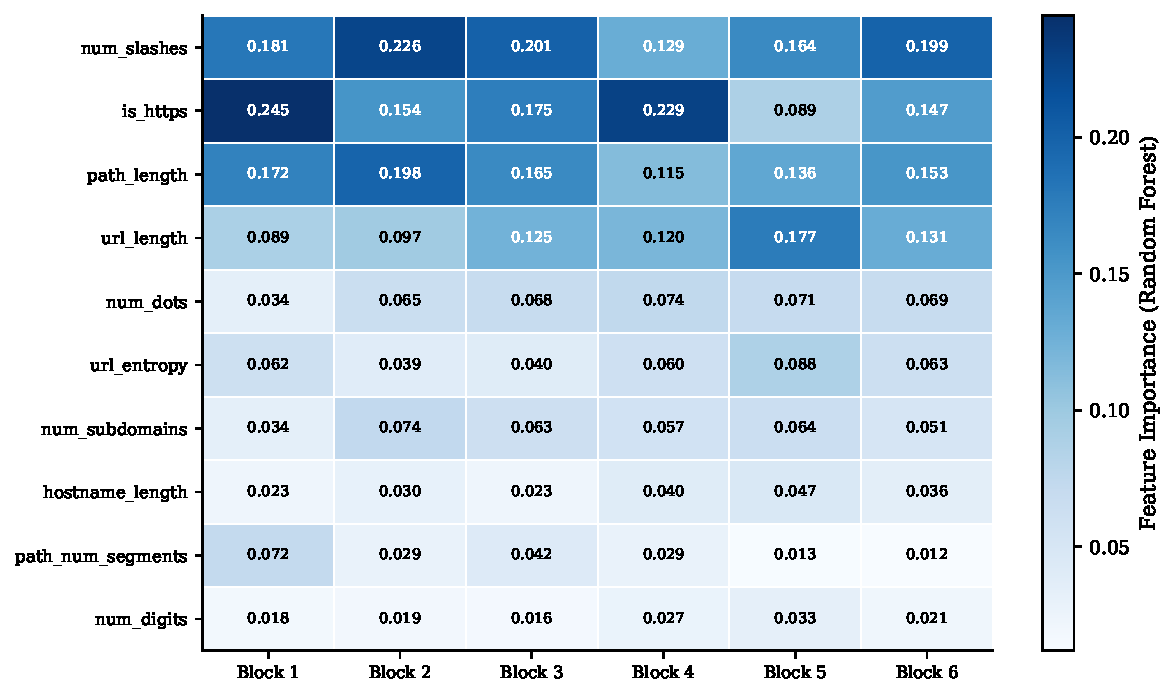
\includegraphics[width=0.75\textwidth]{figures/fig4_importancia_por_bloque.pdf}
\caption{Random forest feature importance by temporal block.}
\label{fig:importancia}
\end{figure}

Direct feature-level evidence supports this reading. The distributional shift in individual lexical features between the earliest and latest temporal blocks is modest, and small compared with the difference between phishing and legitimate URLs (Figure~\ref{fig:desplazamiento}): \texttt{url\_entropy} shows a small rightward shift, but \texttt{url\_length} is essentially unchanged and both \texttt{num\_suspicious\_keywords} and \texttt{has\_ip\_address} remain near-constant, low-variance flags throughout the whole period. Feature importance is correspondingly stable across all six temporal blocks (Figure~\ref{fig:importancia}): \texttt{is\_https}, \texttt{path\_length}, \texttt{num\_slashes}, and \texttt{url\_length} dominate in every block, with no block introducing a qualitatively different top feature. The model is not relying on a fragile, campaign-specific signal that erodes over time; it is relying on a small set of structural URL properties that stay informative because the negative class's lexical signature stays put.

Because these four features are also plausible artifacts of how the legitimate class was constructed (Tranco supplies bare domains, which are structurally shorter and path-free compared to full phishing URLs), we tested whether they are necessary for the near-ceiling performance by re-running the fixed-training design (block 1 versus blocks 2--6) with all four removed, leaving 28 features. Removing the four most important features would lower F1 in almost any problem, so we also removed, as a control, the four most important features that do not depend on whether a URL has a path (\texttt{url\_entropy}, \texttt{num\_dots}, \texttt{num\_subdomains}, \texttt{hostname\_length}). Table~\ref{tab:ablation} shows the result: removing the URL-shape features lowers F1 by 3.3 to 4.2 percentage points (e.g., random forest: 0.9944 to 0.9617 on average across displaced blocks), whereas removing the control features lowers it by 0.05 to 0.38 points. The drop is therefore specific to the features tied to how the legitimate class was built, and part of the near-ceiling result reflects that construction, not phishing-specific content. At the same time, F1 with those four features removed remains at 0.95--0.96, far above chance and only modestly below the full-feature result, so the remaining 28 lexical features carry substantial phishing-discriminating signal on their own. We read this as a partial, not a full, explanation of the near-ceiling result: the four structural features inflate the reported ceiling by a few points, but they are not the sole reason detection is easy.

\begin{table}[h]
\centering
\caption{F1 (fixed-training design, averaged across displaced blocks 2--6) with all 32 features, without the four features tied to legitimate-URL construction (\texttt{is\_https}, \texttt{path\_length}, \texttt{num\_slashes}, \texttt{url\_length}), and without four other important features as a control (\texttt{url\_entropy}, \texttt{num\_dots}, \texttt{num\_subdomains}, \texttt{hostname\_length}). Scaling is fitted on the training block.}
\label{tab:ablation}
\resizebox{\textwidth}{!}{\setlength{\tabcolsep}{7pt}\begin{tabular}{lccccc}
\toprule
 & & \multicolumn{2}{c}{URL-shape features removed} & \multicolumn{2}{c}{Control features removed} \\
\cmidrule(lr){3-4}\cmidrule(lr){5-6}
Model & F1, 32 features & F1 & Drop & F1 & Drop \\
\midrule
Random Forest & 0.9944 & 0.9617 & 0.0327 & 0.9906 & 0.0038 \\
XGBoost & 0.9935 & 0.9601 & 0.0334 & 0.9930 & 0.0005 \\
Logistic Regression & 0.9911 & 0.9492 & 0.0419 & 0.9873 & 0.0038 \\
\bottomrule
\end{tabular}}
\end{table}

The operational risk, then, is not that lexical phishing detectors trained today will fail outright next month. It is that the near-perfect performance reported under a random split (or, as we show, even under most temporal designs against an easy negative class) is a poor guide to performance against near-miss legitimate traffic, which is the regime that actually matters operationally. Whether the degradation trend grows once the negative class is made realistically hard is a question this design cannot answer.

\section{Limitations}

Our features are purely lexical; we do not use page content, WHOIS data, or network/hosting features, all of which could shift the balance between temporal drift and raw separability. PhishTank's reports carry a known reporting-time bias (submission time is not necessarily attack-launch time, and popular/obvious phishing campaigns are reported faster than sophisticated ones). Its downloadable feed also lists only phishing that is still online, so the older blocks contain only the URLs that survived, which are likely to be longer-lived and possibly compromised legitimate sites; time is therefore partly confounded with URL type, and the share of phishing rises across blocks (Data). Prevalence-independent metrics give the same block-level pattern (Results), but the survivorship itself cannot be corrected with this source; a feed archived as it is published would remove it. The 180-day window, while the longest span with consistently high weekly volume in the feed we used, is short relative to multi-year drift dynamics reported elsewhere in the literature. Most importantly, as discussed above, the legitimate-URL sampling from top-ranked Tranco domains very likely understates the real-world temporal degradation a deployed system would face against a harder, more realistic negative class; we consider this the most consequential limitation of the design and the most promising direction for a follow-up study. One further point bears directly on this concern: legitimate URLs receive a synthetic timestamp drawn uniformly over the 180-day window, which makes roughly half of each temporal block i.i.d. with respect to the legitimate class by construction; the small measured degradation could partly reflect this design choice rather than a property of real-world phishing detection. Two of our four designs also confound training-set size with the variable of interest. The random-split baseline in Table~\ref{tab:degradation} trains on 80\% of the full dataset, versus roughly one-sixth (block 1 alone) for the fixed-training design, so part of the random-vs.-temporal gap could reflect the difference in training-set size rather than temporal distance alone; our main degradation-trend analysis relies on the fixed design's within-design trend across distance (constant training set, so this specific confound does not apply there) and on the model-controlled ANCOVA and Page test, not on the random-vs.-fixed comparison itself, but Table~\ref{tab:degradation} is still presented as a headline number and should be read with this caveat. Similarly, cumulative retraining's training set grows with $k$ while sliding-window's stays fixed at one block, so cumulative's small but significant F1 advantage (Results) is also consistent with it simply having more training data at later blocks, rather than simply with retaining older examples being helpful per se. We ran the size-matched control directly: for each evaluation block, training on a stratified random subsample of the cumulative history downsampled to exactly one block's size (10 repetitions per block, averaged), holding training volume fixed at the sliding-window level while varying only which examples (recent-only vs.\ a random historical mix) are included. The result is model-dependent rather than uniform. For random forest, the size-matched F1 (0.9949) differs from sliding-window's (0.9950) by 0.0001 (no test applied), so its cumulative advantage (0.9952) is almost entirely a volume effect. For XGBoost, the size-matched F1 (0.9942) sits roughly halfway between sliding-window (0.9939) and full cumulative (0.9945), splitting the advantage about evenly between volume and a genuine effect of retaining older examples. For logistic regression, the size-matched F1 (0.9916) is \emph{lower} than sliding-window's (0.9923): a random mix of historical examples at fixed volume actively hurts this model relative to training on the most recent block alone, so its full-cumulative advantage (0.9931) comes entirely from added volume, and then some, not from favorable example selection. Retaining historical data is therefore not uniformly beneficial once volume is controlled for; whether it helps, is neutral, or mildly hurts depends on the model family.
\section{Conclusion}

Evaluating three lexical phishing classifiers under four temporal designs on 180 days of PhishTank data, we find a small decline with temporal distance within the fixed-training design that is consistent in direction across models and metrics but not significant when the evaluation block is treated as the independent unit (Spearman $\rho=-0.70$, $p=0.19$), and that cumulative retraining consistently outperforms sliding-window retraining (significant under a paired bootstrap, though not under the underpowered Wilcoxon test), an advantage a size-matched control traces mostly to training-set volume rather than to retaining historical examples per se, with the split between the two explanations itself depending on the model. The magnitude of the effect is modest, well under one F1 point in most configurations, which we attribute chiefly to a negative class (long-established top domains) that is lexically easy to separate from phishing regardless of when the phishing examples were collected, alongside the fact that assigning synthetic timestamps to the legitimate URLs makes half of each evaluation block i.i.d. by construction, which may dilute the observable degradation before any evaluation begins. We recommend that future phishing-detection evaluations pair temporal splitting with a harder negative class before concluding that concept drift is a marginal concern for this task.

\section*{Data Availability}
The PhishTank identifiers and submission times of the phishing URLs (the URLs themselves, which remain malicious links, are not redistributed and can be retrieved from PhishTank by identifier), the sample of legitimate domains with their synthetic timestamps, the extracted feature table, and the analysis code are permanently archived and openly accessible in Zenodo at \url{https://doi.org/10.5281/zenodo.22907771} and GitHub at \url{https://github.com/JuanAvilesP3/phishing-concept-drift}.

\section*{Funding}
This research received no external funding. It was conducted within the academic research framework of Escuela Superior Polit\'ecnica de Chimborazo (ESPOCH).

\section*{Conflict of Interest}
The authors declare that they have no conflict of interest.

\section*{Author Contributions}
\textbf{Juan Pablo Aviles-Esparza:} Conceptualization, Methodology, Software, Writing - Original Draft. \textbf{Italo Javier Tenempaguay-Granizo:} Data Curation, Formal Analysis, Validation, Visualization, Writing - Review \& Editing. \textbf{Isaac David Torres-Paredes:} Supervision, Project Administration, Resources, Writing - Review \& Editing.


\bibliographystyle{ieeetr}
\bibliography{refs}

\end{document}
